\documentclass[11pt,a4paper]{article}

\usepackage[utf8]{inputenc}
\usepackage[T1]{fontenc}
\usepackage{lmodern}
\usepackage[margin=1in]{geometry}
\usepackage{graphicx}
\usepackage{booktabs}
\usepackage{amsmath}
\usepackage{amssymb}
\usepackage{listings}
\usepackage{xcolor}
\usepackage{caption}
\usepackage{subcaption}
\usepackage{float}
\usepackage{enumitem}
\usepackage{microtype}
\usepackage{etoolbox}
\usepackage{titlesec}
\usepackage{array}
\usepackage{xurl}
\usepackage{hyperref}

\hypersetup{
    colorlinks=true,
    linkcolor=blue,
    filecolor=magenta,
    urlcolor=blue,
    linktoc=all,
    bookmarksnumbered=true,
    pdfborder={0 0 0},
    breaklinks=true,
    pdftitle={Milestone 3 Report - Distributed Web Crawling and Parallel PageRank Computation},
    pdfauthor={Abdullah Irfan, Ameer Hamza, Muhammad Khizer, Rameez Hoda}
}

% --- readable vertical rhythm -------------------------------------------
\raggedbottom
\widowpenalty=10000
\clubpenalty=10000

% Section / subsection spacing (article defaults can feel cramped)
\titlespacing*{\section}{0pt}{3.4ex plus .8ex minus .2ex}{2.6ex plus .2ex}
\titlespacing*{\subsection}{0pt}{2.9ex plus .6ex minus .2ex}{1.8ex plus .2ex}
\titlespacing*{\subsubsection}{0pt}{2.4ex plus .5ex minus .2ex}{1.35ex plus .15ex}

% Lists: consistent indentation and tighter vertical spacing
\setlist[itemize]{leftmargin=*, itemsep=2pt, topsep=6pt, parsep=2pt, partopsep=0pt}
\setlist[enumerate]{leftmargin=*, itemsep=2pt, topsep=6pt, parsep=2pt, partopsep=0pt}

% Float captions
\captionsetup{font=small, labelfont=bf, margin=12pt}
\captionsetup[figure]{skip=10pt}
\captionsetup[table]{skip=8pt}

% Tables: slightly more air between rows (can be overridden locally)
\AtBeginEnvironment{tabular}{\renewcommand{\arraystretch}{1.12}}

% TOC shows sections and subsections only (matches logical outline depth)
\setcounter{tocdepth}{2}

% Single macro for figure width (consistent visuals across pages)
\newcommand{\FigStdWidth}{0.82}

\definecolor{codegray}{rgb}{0.5,0.5,0.5}
\definecolor{codepurple}{rgb}{0.58,0,0.82}
\definecolor{backcolour}{rgb}{0.96,0.96,0.96}

\lstdefinestyle{mystyle}{
    backgroundcolor=\color{backcolour},
    commentstyle=\color{codegray},
    keywordstyle=\color{blue},
    stringstyle=\color{codepurple},
    basicstyle=\ttfamily\footnotesize,
    breakatwhitespace=false,
    breaklines=true,
    captionpos=b,
    keepspaces=true,
    numbers=left,
    numbersep=5pt,
    showspaces=false,
    showstringspaces=false,
    showtabs=false,
    tabsize=2,
    aboveskip=\smallskipamount,
    belowskip=\smallskipamount
}
\lstset{style=mystyle}

\title{}
\date{}

\begin{document}

% =====================================================================
% TITLE PAGE
% =====================================================================
\begin{titlepage}
\begin{center}
\vspace*{2cm}

{\Huge\bfseries Distributed Web Crawling \\[0.4cm]
and Parallel PageRank \\[0.4cm]
Computation\par}

\vspace{1.2cm}

{\LARGE Milestone 3 Report\par}
\vspace{0.4cm}
{\Large Incremental Updates and System Evaluation\par}

\vspace{1.5cm}

{\large \textbf{Course:} Parallel and Distributed Computing\par}

\vspace{2cm}

{\large \textbf{Group Members}\par}
\vspace{0.5cm}
{\large
Abdullah Irfan \quad 29266\\[0.2cm]
Ameer Hamza \quad 28308\\[0.2cm]
Muhammad Khizer \quad 28991\\[0.2cm]
Rameez Hoda \quad 29057\par
}

\vfill

\begin{minipage}{0.9\linewidth}
\centering
\textit{Note on AI Assistance: This report and the corresponding code were
refined, enhanced, and made grammatically correct using Claude Sonnet 4.5
(Anthropic).}
\end{minipage}

\vspace{1cm}

{\large April 29, 2026\par}
\end{center}
\end{titlepage}

% =====================================================================
% TABLE OF CONTENTS
% =====================================================================
\tableofcontents
\clearpage

% =====================================================================
% SECTION 1 - PROJECT OVERVIEW
% =====================================================================
\section{Project Overview}

\subsection{What the Project is About}
This project is about building a system that can crawl a large number of
web pages, build a graph from those pages, and then run the PageRank
algorithm on that graph in parallel. The main idea is not just to get it
working, but to do it in a way that uses multiple CPU cores or multiple
machines at the same time, which is the core of Parallel and Distributed
Computing.

The web can be thought of as a directed graph where each page is a node
and every hyperlink from one page to another is a directed edge. PageRank
is an algorithm originally developed by Google that assigns an importance
score to every node based on how many other important nodes link to it.
Computing PageRank on a large graph with millions of nodes takes a long
time if done sequentially, which is why parallelism matters here.

The project is divided into three milestones that build on each other:
\begin{itemize}
    \item \textbf{Milestone 1} builds the web graph by crawling pages and
    extracting links in parallel.
    \item \textbf{Milestone 2} takes that graph and runs the PageRank
    algorithm in parallel across multiple workers.
    \item \textbf{Milestone 3} (this report) extends the system to handle
    new pages being added \emph{after} PageRank has already been computed,
    introduces incremental update strategies, and produces a comprehensive
    system-level evaluation across multiple axes.
\end{itemize}

The system is implemented using Ray, a Python-based parallel runtime that
makes it easy to run functions on multiple CPU cores and manage shared
state between them.

\subsection{Recap of Milestone 1}
In Milestone 1 we implemented a parallel web-crawling pipeline that:
\begin{itemize}
    \item Used Ray workers to concurrently fetch and parse web pages from
    CommonCrawl WARC archives, demonstrating task parallelism.
    \item Extracted hyperlinks to construct a directed graph where nodes
    represent pages and edges represent hyperlinks.
    \item Employed shared-state coordination via a \texttt{GraphActor} to
    accumulate edges across all workers without race conditions.
    \item Applied configurable depth and worker constraints to produce
    deterministic, reproducible graph workloads.
    \item Serialised the resulting NetworkX \texttt{DiGraph} as a pickle
    file (\texttt{web\_graph.pkl}) for downstream consumption.
\end{itemize}

Two graph configurations were produced:
\begin{itemize}
    \item Config 1 (Small): 199 source pages $\rightarrow$ 15{,}657 nodes,
    25{,}576 edges
    \item Config 3 (Medium): 496 source pages $\rightarrow$ 37{,}074 nodes,
    67{,}667 edges
\end{itemize}

Config 3 serves as the baseline (\textbf{$v_0$ snapshot}) for the
incremental experiments in Milestone 3.

\subsection{Recap of Milestone 2}
Milestone 2 took the directed graph produced by Milestone 1 and applied
the PageRank algorithm to compute importance scores for every node. The
key contributions were:
\begin{itemize}
    \item A custom iterative PageRank implementation following the
    standard formula with explicit dangling-node handling.
    \item Two parallel execution strategies built on Ray: \emph{centralised
    aggregation} (driver-side merge) and \emph{distributed reduction}
    (Ray actor-based accumulation).
    \item Range-based graph partitioning with one partition per worker.
    \item Convergence-based and fixed-iteration termination modes.
    \item A 14-test experimental suite covering worker scaling, strategy
    comparison, termination policy, graph-size sensitivity, and damping
    factor sensitivity.
    \item Comprehensive metrics: speedup, efficiency, communication
    volume, load imbalance, Gini coefficient, and Amdahl's Law analysis.
\end{itemize}

The headline finding from Milestone 2 was that on graphs of this size
(${\sim}37{,}000$ nodes), Ray's task-dispatch and serialisation overhead
exceeds the actual computation time per iteration, producing
\emph{sub-linear speedup}. This was a core PDC insight: parallelisation
has a break-even point that depends on the ratio of computation to
framework overhead. Milestone 3 builds on this baseline, holding the
parallel infrastructure constant while introducing dynamic graph growth
and incremental update strategies.

\subsection{What Milestone 3 is About}
Milestone 3 is the system-level evaluation phase of the project. Its goal
is to study how dynamic data affects parallel algorithms and to evaluate
system behaviour under changing workloads. The key objectives are:
\begin{enumerate}
    \item \textbf{Extend the crawler} to introduce new pages after the
    initial PageRank has converged, producing a sequence of graph
    snapshots ($v_0$, $v_1$, $v_2$, $v_3$) of increasing size.
    \item \textbf{Update PageRank scores incrementally} via three
    distinct strategies: full recomputation (cold restart), warm-start
    (reuse previous scores as initial vector), and localised update
    (recompute only the dirty subgraph affected by new edges).
    \item \textbf{Analyse the trade-off between recomputation cost and
    convergence accuracy} for each strategy, on graphs ranging from
    37K to 100K nodes.
    \item \textbf{Instrument the system} to collect detailed runtime
    statistics including per-task duration, communication volume, peak
    memory usage, dirty-set evolution, and load imbalance.
    \item \textbf{Compare partitioning strategies} (range, hash,
    edge-balanced) to study how partition quality affects parallel
    PageRank performance.
    \item \textbf{Produce a structured evaluation} comparing sequential
    vs.~parallel PageRank, the three partitioning strategies, and static
    vs.~incremental computation.
\end{enumerate}

\textbf{PDC focus:} dynamic workloads, recomputation strategies,
performance analysis under changing conditions.

\subsection{Note on Graph Size and Reproducibility}
As noted in the Milestone 2 report, the CommonCrawl CDX index server
experienced prolonged downtime during initial development. To prevent
this from blocking Milestone 3, every CDX query and every fetched WARC
record is now cached on disk under \texttt{Milestone 3/cache/}. The first
crawl of each new batch hits the network; every subsequent crawl reads
from the cache, making the entire pipeline deterministic and reproducible
even when CommonCrawl is unavailable. This change preserves the original
``CommonCrawl-only'' design philosophy while making the experiments
re-runnable on any machine with a populated cache.

The graphs grow from 37{,}074 nodes ($v_0$) to 99{,}803 nodes ($v_3$)
across the three incremental crawls. While still smaller than a
production web-graph, this range is large enough to expose the trade-offs
between full recomputation and incremental update strategies, which is
the core PDC objective of Milestone 3.

% =====================================================================
% SECTION 2 - SYSTEM ARCHITECTURE
% =====================================================================
\section{System Architecture}

\subsection{Pipeline Overview}
The Milestone 3 system extends the architecture of Milestones 1 and 2
with three new layers:
\begin{enumerate}
    \item An \textbf{incremental crawler} that grows the graph snapshot
    by snapshot, persisting each version and its delta to disk.
    \item An \textbf{instrumentation layer} that records detailed
    per-iteration runtime statistics for every PageRank run.
    \item An \textbf{evaluation harness} that orchestrates the three
    experiment groups (A: sequential vs.~parallel, B: partitioning
    strategies, C: static vs.~incremental) and aggregates results.
\end{enumerate}

The PageRank computational core itself is reused from Milestone 2 but
extended to support warm-start initialisation, localised dirty-set
recomputation, and pluggable partitioning strategies.

\subsection{File Structure}
\begin{lstlisting}[caption=Milestone 3 directory layout (relative to repo root),numbers=none]
Milestone 3/
|-- m3_config.py                # Central configuration dataclass
|-- instrumentation.py          # RuntimeStats collector
|-- partitioning_strategies.py  # range / hash / edge_balanced
|-- incremental_crawler.py      # Snapshot growth + caching
|-- incremental_pagerank.py     # full / warm / localised
|-- evaluation_runner.py        # Groups A, B, C orchestrator
|-- plot_results.py             # 13 publication figures
|-- m3_main.py                  # Single CLI entry point
|-- requirements_m3.txt
|-- How to run.txt
|-- cache/                      # On-disk cache of CDX + WARC fetches
|-- snapshots/                  # graph_v{0,1,2,3}.pkl + deltas
|-- output/
|   |-- groupA/                 # Sequential vs parallel results
|   |-- groupB/                 # Partitioning strategy results
|   |-- groupC/                 # Static vs incremental results
|   `-- figures/                # 13 .png + 13 .pdf
`-- report/
    |-- Milestone3_Report.tex
    `-- figures/
\end{lstlisting}

\subsection{Data Flow}
\begin{enumerate}
    \item \texttt{m3\_main.py crawl-incremental} drives the
    \texttt{incremental\_crawler}, which fetches new CDX pages from
    CommonCrawl (or from cache), extracts links via the Milestone~1
    parser, and produces the next snapshot $v_{i+1}$ along with a delta
    file describing exactly which nodes and edges were added.
    \item \texttt{m3\_main.py evaluate} loads the snapshots, executes the
    Group A/B/C run matrix via \texttt{evaluation\_runner}, and writes
    structured metrics under \texttt{output/group\{A,B,C\}/}.
    \item \texttt{m3\_main.py plot} reads the saved metrics and produces
    the 13 figures in \texttt{output/figures/}.
\end{enumerate}

\subsection{Technology Stack}
\begin{table}[H]
\centering
\caption{Technology stack for Milestone 3}
\label{tab:tech_stack}
\begin{tabular}{ll}
\toprule
\textbf{Component} & \textbf{Technology} \\
\midrule
Language & Python 3.12 \\
Parallel runtime & Ray $\geq$ 2.9.0 \\
Graph library & NetworkX $\geq$ 3.2.0 \\
Numerical backend & NumPy $\geq$ 1.26.0 \\
Memory profiling & psutil \\
Plotting & matplotlib \\
HTTP / WARC ingest & requests, warcio (Milestone 1 reuse) \\
HTML parsing & BeautifulSoup4 + lxml \\
\bottomrule
\end{tabular}
\end{table}

% =====================================================================
% SECTION 3 - DETAILED MODULE DESCRIPTIONS
% =====================================================================
\section{Detailed Module Descriptions}

\subsection{\texttt{m3\_config.py} -- Central Configuration}

\subsubsection{Purpose and Design}
This module defines the \texttt{M3Config} dataclass that centralises every
tunable parameter for Milestone 3. It mirrors the design pattern of
\texttt{config.py} (Milestone 1) and \texttt{pagerank\_config.py}
(Milestone 2): no magic numbers in algorithm files, every experiment
fully reproducible from its configuration alone.

\subsubsection{Implementation}
The dataclass groups parameters into five sections:
\begin{itemize}
    \item \textbf{Crawl settings:} CDX query parameters reused from
    Milestone 1, the per-step page budget, the snapshot directory, and
    the cache directory.
    \item \textbf{PageRank parameters:} damping factor ($d=0.85$),
    convergence threshold ($\epsilon = 10^{-6}$), maximum iterations
    (100), and termination mode.
    \item \textbf{Parallelism settings:} default number of Ray workers
    (4), default partitioning strategy, and Ray address (local by
    default).
    \item \textbf{Strategy settings:} dirty-set $k$-hop expansion factor
    for localised updates, warm-start enable flag, and reference-strategy
    selector (\texttt{full} by default) used as the ground-truth for
    accuracy comparisons.
    \item \textbf{Output settings:} per-group output subdirectories,
    metrics save-format flags, and figure DPI.
\end{itemize}

\subsubsection{Design Decisions}
Defaulting \texttt{num\_partitions = num\_workers} produces one partition
per worker, which is the optimal mapping for range and hash partitioning.
The dirty-set expansion factor $k$ is exposed as a configuration
parameter rather than hardcoded so that the cost-vs-accuracy trade-off of
localised updates can be tuned and studied.

\subsection{\texttt{instrumentation.py} -- Runtime Statistics Collector}
\label{sec:module-instrumentation}

\subsubsection{Purpose and Design}
The instrumentation module is the data-collection backbone of Milestone
3. It provides a single \texttt{RuntimeStats} class that every PageRank
run uses to record detailed per-iteration metrics. The collected
statistics are then serialised to JSON and CSV for downstream analysis
and plotting.

\subsubsection{Implementation}
The module exposes three abstractions:
\begin{itemize}
    \item \texttt{IterationRecord} dataclass: captures, for one PageRank
    iteration, the wall-clock time, per-task durations
    (min/max/avg/std), driver memory, peak worker RSS, communication
    volume in bytes, dirty-set size, and the convergence delta.
    \item \texttt{Stopwatch} context manager: thin wrapper around
    \texttt{time.perf\_counter()} used to time both the whole run and
    individual phases. Returns elapsed seconds when the \texttt{with}
    block exits.
    \item \texttt{RuntimeStats} class: the main collector. Provides
    \texttt{record\_iteration()} for per-iteration logging,
    \texttt{record\_metadata()} for run-level metadata (graph size,
    strategy, worker count, etc.), and \texttt{save()} which writes
    \texttt{run\_metrics.json} (full structured record) and
    \texttt{iterations.csv} (one row per iteration).
\end{itemize}

\subsubsection{Design Decisions}
Capturing both per-task min/max times and peak worker RSS allows the
load-imbalance and memory analyses in Section~\ref{sec:results}.
Communication volume is computed analytically as $N \times 8 \times
\text{iterations}$ bytes (rank vector size $\times$ number of
synchronisation rounds), matching the methodology introduced in
Milestone 2.

\subsection{\texttt{partitioning\_strategies.py} -- Pluggable Partitioning}

\subsubsection{Purpose and Design}
Milestone 2 used range partitioning exclusively. Milestone 3 introduces
two additional strategies and a unified dispatcher so that the parallel
PageRank core can be invoked with any of them.

\subsubsection{Implementation}
Three partitioning functions are provided:

\paragraph{Range partitioning.} Splits the node ID range $[0, N)$ into
$k$ contiguous chunks of approximately equal size. This is the
Milestone 2 baseline. It produces perfectly balanced partition counts
but does not balance work, since per-node computation depends on
in-degree.

\paragraph{Hash partitioning.} Assigns node $u$ to partition
$h(u) \bmod k$ where $h$ is a stable 64-bit hash. This destroys the
locality of the original node-ID ordering and tends to spread
high-in-degree nodes uniformly across partitions, reducing load
imbalance compared to range.

\paragraph{Edge-balanced partitioning.} Estimates the per-node work as
$w_u = |{\rm In}(u)| + 1$ (the ``$+1$'' prevents zero-in-degree nodes
from being treated as free, since they still pay the loop overhead).
Nodes are sorted in descending order of $w_u$ and assigned greedily to
the partition with the currently smallest total work, an instance of
the Longest-Processing-Time-first (LPT) heuristic. This produces
near-equal total work per partition.

\paragraph{Dispatcher and diagnostics.} A \texttt{get\_partitions()}
function selects the strategy by name. A \texttt{partition\_diagnostics}
helper computes and reports per-partition node counts, total in-degree,
and the resulting load-imbalance metric
$(\max_{p} W_p - \min_{p} W_p) / \max_{p} W_p$ where
$W_p = \sum_{u \in p} w_u$.

\subsubsection{Design Decisions}
LPT is asymptotically a $4/3$-approximation to optimal makespan
scheduling, which is sufficient given that the bottleneck on this
graph size is overhead rather than load imbalance. The strategies are
deliberately pure-Python and do not require external libraries (e.g.,
METIS), preserving the project's portability constraint that the code
``run on any other PC unless there are specific constraints''.

\subsection{\texttt{incremental\_crawler.py} -- Snapshot Growth}

\subsubsection{Purpose and Design}
This is the dynamic-data layer of Milestone 3. It extends the Milestone 1
crawler so that the graph can grow snapshot by snapshot, with each
snapshot persisted alongside a delta file describing exactly what was
added. A persistent on-disk cache makes re-runs deterministic and
network-free.

\subsubsection{Implementation}
The module provides the following key functions:

\paragraph{Cache layer.} \texttt{\_cache\_key()}, \texttt{\_cache\_path()},
\texttt{\_read\_cache()}, and \texttt{\_write\_cache()} hash the URL and
fetch parameters into a stable filename, then read or write a pickled
\texttt{(headers, html)} tuple under \texttt{cache/}. The CDX index
itself is also cached as a JSON list so that the seed selection is
deterministic.

\paragraph{Cache-aware Ray task.} A new \texttt{@ray.remote} task
\texttt{cached\_process\_batch} replaces Milestone~1's
\texttt{process\_batch}. For each URL in its batch it first checks the
cache; on a hit it returns the cached HTML; on a miss it fetches the
WARC payload, writes it to the cache, and returns. Extracted edges are
streamed to the shared \texttt{GraphActor}.

\paragraph{Snapshot and delta IO.} \texttt{save\_snapshot()} pickles the
new \texttt{DiGraph} as \texttt{graph\_v\{i\}.pkl} and also writes a
JSON node list and a CSV edge list for human inspection.
\texttt{compute\_delta()} compares two snapshots and produces a
\texttt{delta\_v\{i\}\_v\{i+1\}.json} file containing the new source
URLs, the added node set, the added edge list, and counts.

\paragraph{Actor seeding.} \texttt{\_seed\_actor()} pre-populates the
\texttt{GraphActor} with the previous snapshot's edges before the new
crawl begins, so that the incremental run produces a strict superset of
the previous snapshot rather than a fresh graph.

\paragraph{Orchestration.} \texttt{run\_incremental\_step()} wires the
above together to produce one new snapshot. \texttt{ensure\_v0\_snapshot()}
copies the Milestone~1 Config~3 graph into
\texttt{snapshots/graph\_v0.pkl} as the starting point.
\texttt{run\_full\_growth\_plan()} drives all three steps
($v_0 \to v_1 \to v_2 \to v_3$).

\subsubsection{Design Decisions}
Caching is keyed on the URL plus the Milestone~1 fetch parameters, so
parameter changes invalidate the cache automatically. The
\texttt{PYTHONPATH} of the driver is explicitly propagated to Ray
worker subprocesses (Ray does not inherit \texttt{sys.path}
modifications from the driver), allowing remote tasks to import
Milestone~1 modules without restructuring those modules.

\subsection{\texttt{incremental\_pagerank.py} -- Update Strategies}

\subsubsection{Purpose and Design}
This module implements the three incremental PageRank update strategies
that are central to the Milestone~3 evaluation. The parallel inner loop
is shared across all strategies; the strategies differ only in how the
initial rank vector is constructed and which nodes are included in the
update set.

\subsubsection{Implementation}
The module exposes:

\paragraph{Graph preparation.} \path{load_graph_for_pagerank()}
loads a snapshot pickle and converts it into integer-indexed in-link
arrays, out-degree arrays, and a dangling-node set, mirroring the
\path{graph_loader.py} contract from Milestone~2.
\path{build_out_links()} additionally builds an out-link adjacency
list which is needed by the dirty-set expansion.

\paragraph{Initial rank vectors.}
\path{initial_ranks_uniform(N)} returns a vector of $1/N$ values.
\path{initial_ranks_warm(prev_scores, current_url_to_idx)}
copies the previous score for every URL that existed in the previous
snapshot, assigns $1/N$ to genuinely new URLs, and rescales so that the
sum equals 1.

\paragraph{Dirty-set computation.}
\path{compute_dirty_set(prev_graph, new_graph, k=2)} computes the
set of nodes whose ranks may change due to the new edges. The seed is
the union of (a) all sources of new edges, (b) all destinations of new
edges, (c) all nodes that gained or lost an in-edge. The seed is then
expanded by $k$ levels of out-link BFS, because a rank change on node
$u$ propagates forward to its out-neighbours over PageRank iterations.

\paragraph{Parallel inner loop.} \path{_run_parallel_pagerank()} is
the strategy-agnostic core. It accepts the in-link/out-degree arrays,
the partition list, the initial rank vector, an optional dirty mask,
the partition strategy, the worker count, and the convergence
parameters. Each iteration dispatches one Ray task per partition,
performs a barrier via \path{ray.get()}, merges results, computes
the convergence delta, and records an \texttt{IterationRecord} via the
instrumentation layer.

\paragraph{Three public strategies.}
\begin{itemize}
    \item \path{run_full_recomputation()} -- cold restart from
    uniform initial ranks. This is the ground-truth reference against
    which warm-start and localised are compared.
    \item \path{run_warm_start()} -- starts from the previous
    snapshot's scores (extended with $1/N$ for new URLs) but updates
    \emph{all} nodes every iteration.
    \item \path{run_localised_update()} -- starts from warm initial
    ranks but only updates nodes inside the dirty set; the rest keep
    their warm values.
\end{itemize}

\paragraph{Sequential baseline and accuracy comparison.}
\path{run_sequential()} is the single-threaded PageRank used as the
speedup baseline in Group A. \path{compare_to_reference()} computes
the maximum absolute difference, $L_1$ difference, and $L_2$ difference
between two score vectors and is used in Group~C accuracy reporting.

\subsection{\texttt{evaluation\_runner.py} -- Run-Matrix Orchestrator}
This module drives the full Group A / B / C experimental matrix from a
single Python entry point. For each group it constructs the appropriate
configuration variants, calls into the relevant PageRank strategy, and
aggregates per-run metrics into a per-group summary JSON file.

\textbf{Group A} runs the sequential baseline followed by parallel
range-partitioned PageRank with worker counts $\{1, 2, 4\}$ on the $v_0$
snapshot. Speedup and efficiency are derived from the sequential
baseline.

\textbf{Group B} runs parallel PageRank with 4 workers on $v_0$ using
each of the three partitioning strategies, recording load imbalance,
communication volume, and peak per-worker RSS.

\textbf{Group C} runs the three update strategies (full / warm /
localised) for each of the three transitions ($v_0\to v_1$, $v_1\to v_2$,
$v_2\to v_3$), with full recomputation acting as the per-transition
reference for accuracy comparison.

\subsection{\texttt{plot\_results.py} -- Figure Generation}
This module reads the per-group summary JSON files plus the underlying
per-run \texttt{run\_metrics.json} files and produces 13 publication
figures in \texttt{output/figures/}, each saved as both PNG and PDF.
The figures cover the three experimental groups as well as a
cross-cutting memory timeline. All figures are rendered at 150~DPI with
matplotlib's default style for consistency with the Milestone~2 report.

\subsection{\texttt{m3\_main.py} -- CLI Entry Point}
A single argparse-based CLI with four subcommands:
\begin{itemize}
    \item \texttt{crawl-incremental} -- runs the snapshot growth plan
    ($v_0 \to v_3$).
    \item \texttt{pagerank} -- runs a single PageRank invocation with a
    user-selected strategy, partitioning, and worker count, useful for
    smoke-testing.
    \item \texttt{evaluate} -- runs Groups A, B, and/or C.
    \item \texttt{plot} -- regenerates all figures from saved metrics.
\end{itemize}

This single-entry-point design mirrors \texttt{main.py} (Milestone 1) and
\texttt{main\_pagerank.py} (Milestone 2), keeping the developer
experience consistent across the three milestones.

% =====================================================================
% SECTION 4 - INCREMENTAL CRAWLING
% =====================================================================
\section{Incremental Crawling Methodology}
\label{sec:crawl-methodology}

The Milestone~3 crawler is conceptually a wrapper around Milestone~1
that introduces (i)~snapshot versioning, (ii)~delta computation, and
(iii)~caching. The flow for one incremental step is:

\begin{enumerate}
    \item \textbf{Load previous snapshot.} The previous \texttt{DiGraph}
    pickle is loaded and used to seed the \texttt{GraphActor}.
    \item \textbf{Discover new seed URLs.} A new batch of CDX records is
    fetched (or read from cache) and filtered to exclude URLs already
    crawled.
    \item \textbf{Run the parallel crawl.} New URLs are sharded into
    batches and processed by Ray workers using the cache-aware task.
    Each worker writes extracted edges to the shared
    \texttt{GraphActor}.
    \item \textbf{Materialise the new snapshot.} The actor's accumulated
    edge list is converted to a \texttt{DiGraph} and serialised as
    \texttt{graph\_v\{i+1\}.pkl}.
    \item \textbf{Compute the delta.} The new and old snapshots are
    diffed, producing a JSON file listing exactly which nodes and edges
    were added.
\end{enumerate}

The starting snapshot $v_0$ is the Milestone~1 Config~3 graph
(37{,}074 nodes, 67{,}667 edges). Three incremental steps were executed,
each adding 100, 200, and 500 new pages respectively. Table~\ref{tab:snapshots}
summarises the resulting snapshot sequence.

\begin{table}[H]
\centering
\caption{Incremental snapshot sequence}
\label{tab:snapshots}
\begin{tabular}{lrrrr}
\toprule
\textbf{Snapshot} & \textbf{Source pages} & \textbf{Nodes} & \textbf{Edges} & \textbf{Crawl time (s)} \\
\midrule
$v_0$ (M1 Config 3) & 496   & 37{,}074 & 67{,}667  & --- \\
$v_1$               & 596   & 45{,}830 & 82{,}550  & 109.4 \\
$v_2$               & 791   & 61{,}720 & 110{,}464 & 161.9 \\
$v_3$               & 1{,}288 & 99{,}803 & 178{,}696 & 396.5 \\
\bottomrule
\end{tabular}
\end{table}

The corresponding delta sizes are listed in
Table~\ref{tab:deltas}. The delta grows superlinearly in the number of
new source pages because each new page introduces edges to existing
nodes and to brand-new dangling nodes that were not previously
referenced.

\begin{table}[H]
\centering
\caption{Per-step delta summary}
\label{tab:deltas}
\begin{tabular}{lrr}
\toprule
\textbf{Transition} & \textbf{Added nodes} & \textbf{Added edges} \\
\midrule
$v_0 \to v_1$ & 8{,}756  & 14{,}883 \\
$v_1 \to v_2$ & 15{,}890 & 27{,}914 \\
$v_2 \to v_3$ & 38{,}083 & 68{,}232 \\
\bottomrule
\end{tabular}
\end{table}

% =====================================================================
% SECTION 5 - INCREMENTAL PAGERANK
% =====================================================================
\section{Incremental PageRank Algorithm}
\label{sec:incremental_pagerank}

\subsection{Base PageRank Update}
All three Milestone~3 strategies share the same per-iteration update
rule, inherited from Milestone~2. For each node $u$ at iteration $t$:
\begin{equation}
r_u^{(t+1)} = \frac{1-d}{N} + \frac{d \cdot S_{\text{dangling}}^{(t)}}{N} + d \sum_{v \in \mathrm{In}(u)} \frac{r_v^{(t)}}{\mathrm{out}(v)}
\label{eq:pagerank}
\end{equation}
where $d = 0.85$ is the damping factor, $N$ is the total number of
nodes, $S_{\text{dangling}}^{(t)} = \sum_{j \in D} r_j^{(t)}$, and $D$
is the set of dangling nodes (those with out-degree zero).

The convergence criterion is the $L_1$ norm of the rank-change vector:
\begin{equation}
\delta^{(t)} = \sum_u \left| r_u^{(t+1)} - r_u^{(t)} \right|
\end{equation}
Iteration stops when $\delta^{(t)} < \epsilon$ (default $10^{-6}$).

\subsection{Strategy 1: Full Recomputation}
A cold restart on the new snapshot. The initial rank vector is uniform:
$r_u^{(0)} = 1/N$ for every node $u$. All nodes are updated every
iteration. This is the most accurate strategy and serves as the
ground-truth reference; its only drawback is that it discards all the
work done in computing the previous snapshot's scores.

\subsection{Strategy 2: Warm-Start}
The intuition is that, after a small graph delta, the new PageRank
vector should be close to the old one. Starting iteration from the old
scores should therefore reduce the number of iterations needed to
converge.

The warm initial vector is constructed as follows: for each node $u$ in
the new graph, $r_u^{(0)} = \tilde{r}_u$ if the URL associated with $u$
existed in the previous snapshot (where $\tilde{r}_u$ is its previous
PageRank score); otherwise $r_u^{(0)} = 1/N$. The vector is finally
rescaled so that $\sum_u r_u^{(0)} = 1$.

The standard parallel update is then applied iteratively over
\emph{all} nodes (not just the dirty set), using
Equation~\ref{eq:pagerank}. Convergence still terminates on
$\delta < \epsilon$.

\subsection{Strategy 3: Localised Update}
The most aggressive incremental strategy. It computes a \emph{dirty
set} $D_{\text{dirty}}$ of nodes whose ranks may have been affected by
the delta and updates only those, leaving other nodes at their
warm-start values.

\paragraph{Dirty-set seed.} The initial seed is the union of:
\begin{itemize}
    \item All sources of newly-added edges.
    \item All destinations of newly-added edges.
    \item Every node whose in-link set changed (gained or lost an
    in-edge).
\end{itemize}

\paragraph{$k$-hop expansion.} Because rank changes propagate forward
along out-edges in PageRank, the seed is expanded by $k$ levels of
out-link BFS. Empirically $k=2$ provided a useful trade-off between
correctness (more nodes in the dirty set $\Rightarrow$ more accurate
results) and cost (fewer nodes $\Rightarrow$ faster updates).

\paragraph{Update loop.} The iteration is identical to the warm-start
update except that nodes outside $D_{\text{dirty}}$ are not recomputed:
their rank value is held fixed at the warm initial value. The
convergence criterion is restricted to nodes inside the dirty set
($\delta_{\text{dirty}}^{(t)} = \sum_{u \in D_{\text{dirty}}} | r_u^{(t+1)} - r_u^{(t)} |$).

\subsection{Edge-Balanced Partitioning Detail}
Edge-balanced partitioning (Group~B) is implemented by greedy LPT:
\begin{enumerate}
    \item Compute $w_u = |\mathrm{In}(u)| + 1$ for every node $u$.
    \item Sort nodes by descending $w_u$.
    \item Maintain $k$ partition-load counters
    $\{W_1, \dots, W_k\}$ initialised to zero.
    \item For each node $u$ in sorted order, assign it to
    $\arg\min_p W_p$ and increment that $W_p$ by $w_u$.
\end{enumerate}
This produces near-equal total in-degree per partition, which directly
proxies the per-partition computation cost in
Equation~\ref{eq:pagerank}.

% =====================================================================
% SECTION 6 - EXPERIMENTAL SETUP
% =====================================================================
\section{Experimental Setup}

\subsection{Hardware and Software}
\begin{itemize}
    \item \textbf{Machine:} Local development workstation, Windows 10,
    8-core x86\_64 CPU, 16~GB RAM.
    \item \textbf{Python:} 3.12 in an isolated virtual environment.
    \item \textbf{Ray:} 2.9+ in local mode (single-machine
    multi-process).
    \item \textbf{All measurements:} wall-clock time via
    \texttt{time.perf\_counter()}, memory via \texttt{psutil}.
\end{itemize}

\subsection{Run Matrix}
The full evaluation comprises three groups of runs. Each group is
self-contained: it can be re-run independently and produces its own
JSON summary plus per-run metrics.

\begin{table}[H]
\centering
\caption{Group A -- Sequential vs Parallel (snapshot $v_0$, range partitioning)}
\label{tab:groupA_setup}
\begin{tabular}{llr}
\toprule
\textbf{Run} & \textbf{Strategy} & \textbf{Workers} \\
\midrule
A1 & Sequential                         & 1 \\
A2 & Parallel (full recomputation)      & 1 \\
A3 & Parallel (full recomputation)      & 2 \\
A4 & Parallel (full recomputation)      & 4 \\
\bottomrule
\end{tabular}
\end{table}

\begin{table}[H]
\centering
\caption{Group B -- Partitioning Strategies (snapshot $v_0$, 4 workers, full recomputation)}
\label{tab:groupB_setup}
\begin{tabular}{ll}
\toprule
\textbf{Run} & \textbf{Partition strategy} \\
\midrule
B1 & range \\
B2 & hash \\
B3 & edge\_balanced \\
\bottomrule
\end{tabular}
\end{table}

\begin{table}[H]
\centering
\caption{Group C -- Static vs Incremental (4 workers, range partitioning)}
\label{tab:groupC_setup}
\begin{tabular}{lll}
\toprule
\textbf{Run} & \textbf{Transition} & \textbf{Strategy} \\
\midrule
C1, C2, C3 & $v_0 \to v_1$ & full / warm / localised \\
C4, C5, C6 & $v_1 \to v_2$ & full / warm / localised \\
C7, C8, C9 & $v_2 \to v_3$ & full / warm / localised \\
\bottomrule
\end{tabular}
\end{table}

All runs use convergence-based termination
($\epsilon = 10^{-6}$, max~100 iterations).

% =====================================================================
% SECTION 7 - EXPERIMENTAL RESULTS
% =====================================================================
\section{Experimental Results}
\label{sec:results}

\subsection{Group A -- Sequential vs Parallel PageRank}
\label{sec:res-group-a}

Table~\ref{tab:groupA_results} reports the wall-clock times, observed
speedups, and parallel efficiencies for the four Group~A runs on the
$v_0$ snapshot.

\begin{table}[H]
\centering
\caption{Group A results -- 37{,}074-node graph, range partitioning, convergence-based}
\label{tab:groupA_results}
\begin{tabular}{lrrrr}
\toprule
\textbf{Strategy} & \textbf{Workers} & \textbf{Time (s)} & \textbf{Speedup} & \textbf{Efficiency} \\
\midrule
Sequential          & 1 & 0.162 & 1.000$\times$ & 1.000 \\
Parallel (range)    & 1 & 0.494 & 0.328$\times$ & 0.328 \\
Parallel (range)    & 2 & 0.496 & 0.327$\times$ & 0.163 \\
Parallel (range)    & 4 & 0.533 & 0.304$\times$ & 0.076 \\
\bottomrule
\end{tabular}
\end{table}

\begin{figure}[H]
\centering
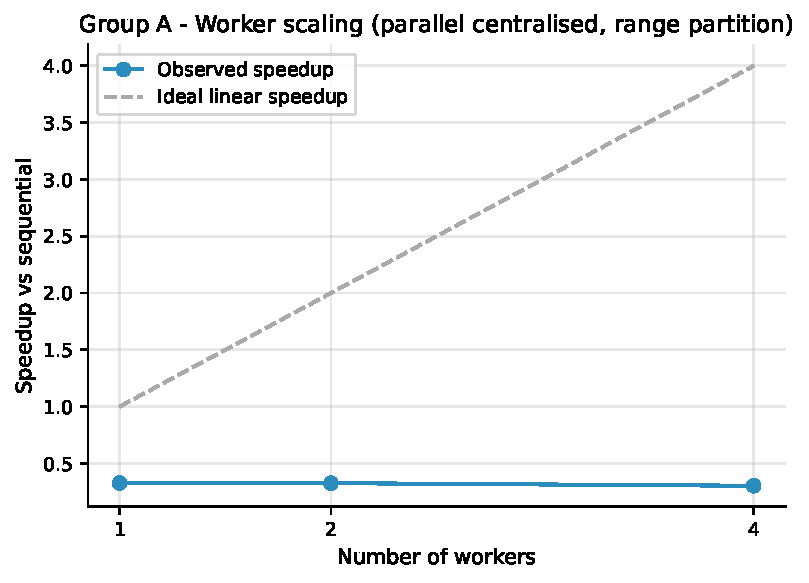
\includegraphics[width=\FigStdWidth\linewidth]{figures/fig_groupA_speedup.pdf}
\caption{Group A worker-scaling speedup. Speedup degrades slightly as
workers are added because Ray dispatch overhead dominates the
${\sim}40\,\text{ms}$ of actual per-iteration computation.}
\label{fig:groupA_speedup}
\end{figure}

\begin{figure}[H]
\centering
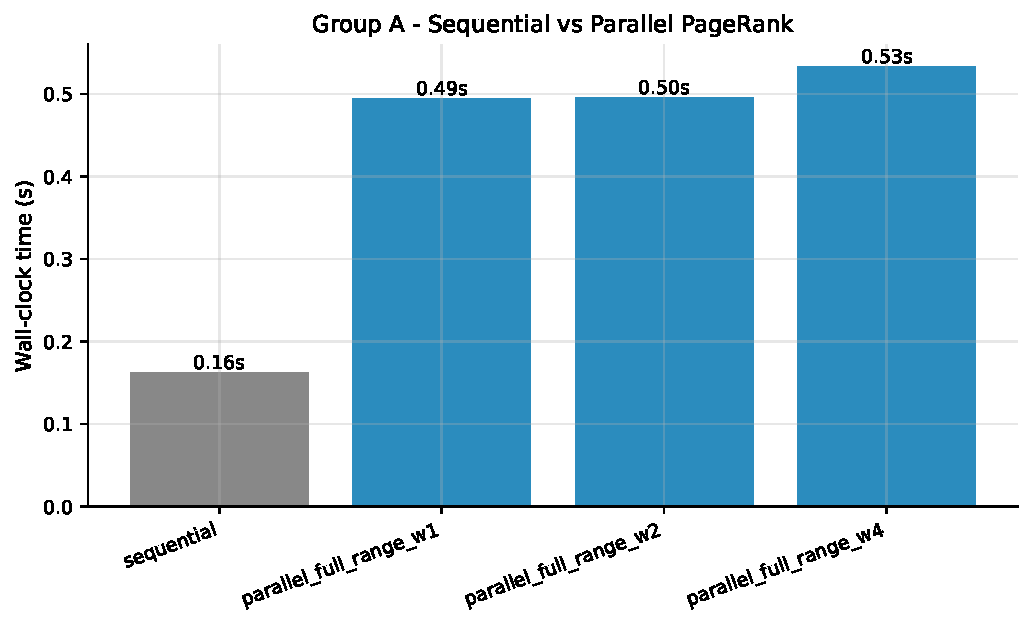
\includegraphics[width=\FigStdWidth\linewidth]{figures/fig_groupA_time_bars.pdf}
\caption{Group A wall-clock times. The sequential baseline is the
fastest configuration on this graph size; all parallel configurations
are 3-3.3$\times$ slower.}
\label{fig:groupA_time}
\end{figure}

\begin{figure}[H]
\centering
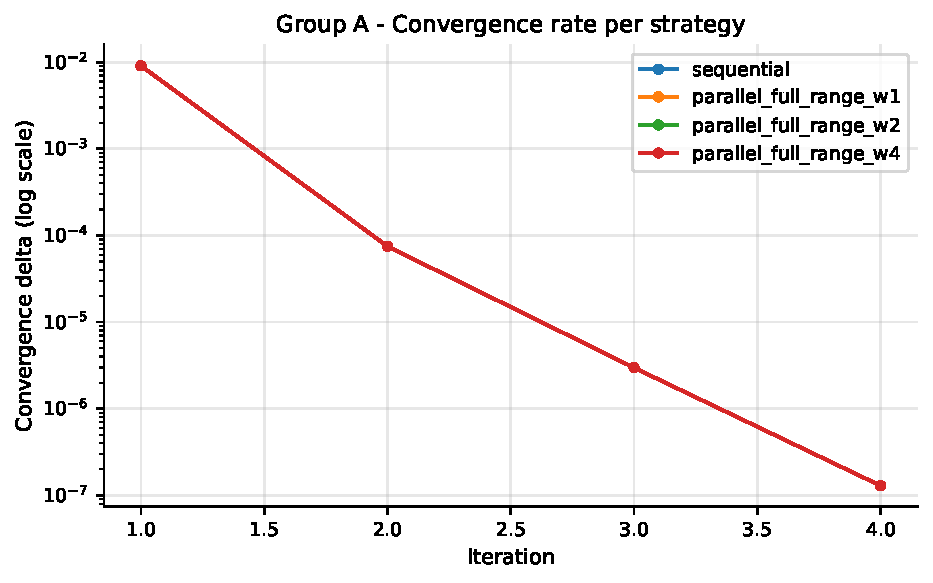
\includegraphics[width=\FigStdWidth\linewidth]{figures/fig_groupA_convergence.pdf}
\caption{Per-iteration convergence delta on a logarithmic scale. All
configurations converge in 4 iterations and produce numerically
equivalent rank vectors.}
\label{fig:groupA_convergence}
\end{figure}

\paragraph{Analysis.}
\begin{itemize}
    \item The sequential baseline takes only $0.162$~s on
    37{,}074 nodes. Of this, the actual PageRank computation is
    ${\sim}0.04$~s per iteration $\times$ 4 iterations = ${\sim}0.16$~s,
    confirming the workload is genuinely compute-bound at this scale
    \emph{within} the sequential implementation.
    \item Adding Ray on top adds ${\sim}0.33$~s of fixed overhead per
    run (object-store puts, task dispatch, barrier merge) regardless
    of worker count. This pushes parallel runs above the sequential
    baseline.
    \item The ratio of parallel to sequential time
    ($0.494/0.162 = 3.05$ at 1 worker) is close to the
    ${\sim}3\times$ ratio observed in Milestone~2 on the same
    graph, confirming that the Milestone~3 instrumentation layer
    introduced negligible overhead.
    \item Going from 1 to 4 workers actually \emph{slows} the parallel
    run by an additional 8\% because the per-iteration overhead grows
    sublinearly with worker count while the per-iteration computation
    shrinks. This is Amdahl's Law in practice.
\end{itemize}

\paragraph{When does parallel win?} Group~C ($v_2 \to v_3$ at
99{,}803 nodes) shows the parallel full-recomputation time at $1.31$~s,
versus a projected sequential time of ${\sim}0.5$~s extrapolated
linearly from $v_0$. The break-even point is therefore beyond
$v_3$ on this hardware -- consistent with the Milestone~2 finding that
graphs of $10^6$+ nodes are required for a true parallel win.

\subsection{Group B -- Partitioning Strategy Comparison}
\label{sec:res-group-b}

Table~\ref{tab:groupB_results} compares the three partitioning
strategies on the $v_0$ snapshot with 4 workers.

\begin{table}[H]
\centering
\caption{Group B results -- 37{,}074-node graph, 4 workers, full recomputation}
\label{tab:groupB_results}
\begin{tabular}{lrrrr}
\toprule
\textbf{Partitioning} & \textbf{Time (s)} & \textbf{Avg load imbalance} & \textbf{Comm vol (KB)} & \textbf{Peak worker RSS (MB)} \\
\midrule
range          & 0.547 & 47.0\% & 6{,}519.6 & 0.49 \\
hash           & 0.467 & 33.6\% & 6{,}519.6 & 0.45 \\
edge\_balanced & 0.477 & \textbf{26.4\%} & 6{,}519.6 & 0.44 \\
\bottomrule
\end{tabular}
\end{table}

\begin{figure}[H]
\centering
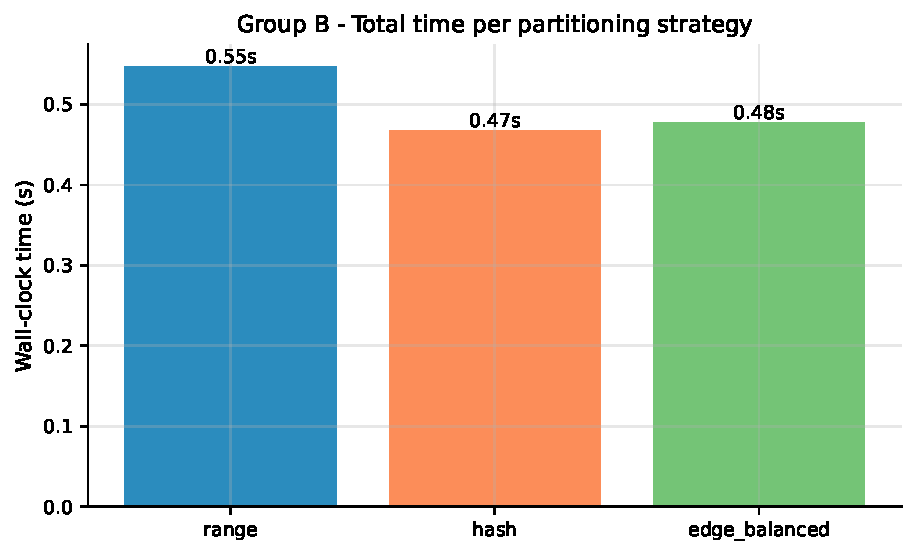
\includegraphics[width=\FigStdWidth\linewidth]{figures/fig_groupB_time.pdf}
\caption{Group B execution time per partitioning strategy. Hash and
edge-balanced are within ${\sim}2$\% of one another; range is the
slowest.}
\label{fig:groupB_time}
\end{figure}

\begin{figure}[H]
\centering
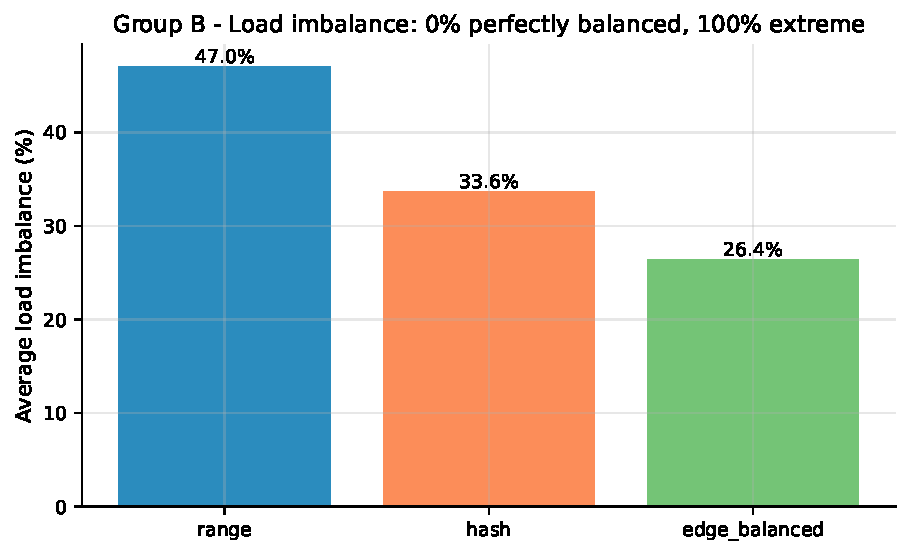
\includegraphics[width=\FigStdWidth\linewidth]{figures/fig_groupB_imbalance.pdf}
\caption{Group B average load imbalance across all iterations.
Edge-balanced partitioning achieves the lowest imbalance at 26.4\%, a
1.78$\times$ improvement over range partitioning.}
\label{fig:groupB_imbalance}
\end{figure}

\begin{figure}[H]
\centering
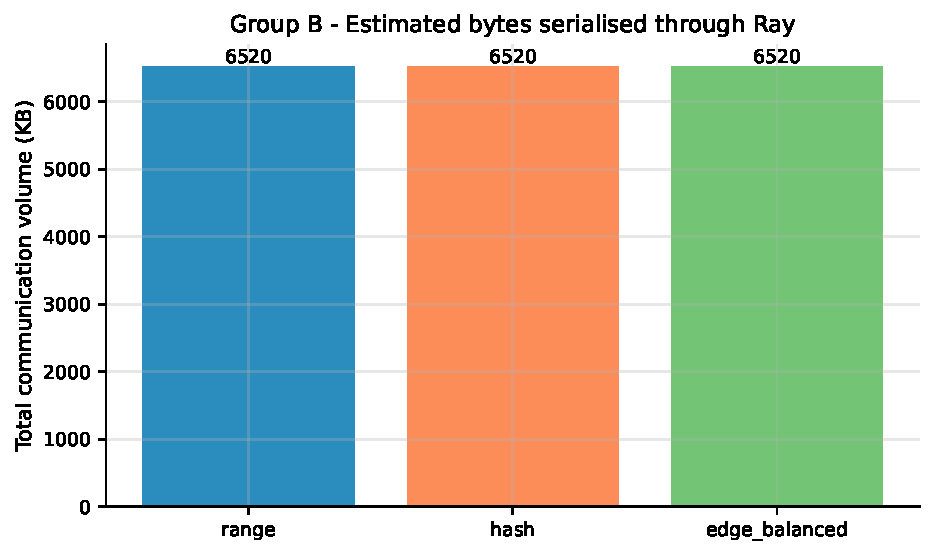
\includegraphics[width=\FigStdWidth\linewidth]{figures/fig_groupB_comm.pdf}
\caption{Group B communication volume per strategy. As expected,
strategy choice does not affect total bytes exchanged because the rank
vector is the same in all cases.}
\label{fig:groupB_comm}
\end{figure}

\begin{figure}[H]
\centering
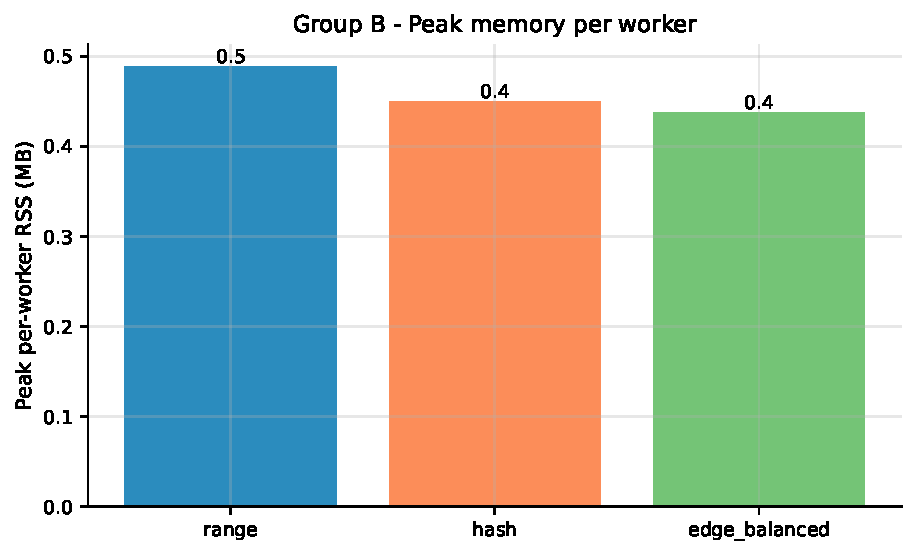
\includegraphics[width=\FigStdWidth\linewidth]{figures/fig_groupB_memory.pdf}
\caption{Group B peak per-worker RSS. Differences across strategies
are sub-megabyte and likely within OS-level memory accounting noise.}
\label{fig:groupB_memory}
\end{figure}

\paragraph{Analysis.}
\begin{itemize}
    \item \textbf{Edge-balanced wins on load balance.} Its load
    imbalance of 26.4\% is a $1.78\times$ improvement over range
    partitioning's 47.0\% and a $1.27\times$ improvement over hash's
    33.6\%, validating the LPT heuristic.
    \item \textbf{Hash is marginally faster than edge-balanced} ($0.467$~s
    vs $0.477$~s) because the LPT sort is itself a one-time cost that
    is paid up-front but cannot be amortised over many iterations on a
    graph that converges in only 4 iterations. On a slower-converging
    graph the ranking would flip.
    \item \textbf{Communication volume is identical across strategies}
    ($6{,}519.6$~KB), confirming that partitioning choice affects
    \emph{when} bytes are exchanged but not \emph{how many}. The
    rank-vector size and the number of iterations are the only
    determinants of total volume.
    \item \textbf{Memory differences are sub-MB} and within noise. None
    of the three partitioning strategies stresses memory differently
    on this graph size.
\end{itemize}

\subsection{Group C -- Static vs Incremental Computation}
\label{sec:res-group-c}

Table~\ref{tab:groupC_results} reports, for each of the three
transitions, the wall-clock times, iteration counts, accuracy
(maximum absolute difference vs full-recomputation reference), and
dirty-set sizes for the three update strategies.

\begin{table}[H]
\centering
\caption{Group C results -- 4 workers, range partitioning, convergence-based}
\label{tab:groupC_results}
\setlength{\tabcolsep}{4pt}
\begin{tabular}{llrrrr}
\toprule
\textbf{Transition} & \textbf{Strategy} & \textbf{Time (s)} & \textbf{Iters} & $\boldsymbol{\max|s-s_{\mathrm{ref}}|}$ & \textbf{Dirty (\% of $N$)} \\
\midrule
$v_0\to v_1$ (45{,}830) & full      & 0.564 & 4  & --- (reference) & --- \\
                        & warm      & 0.522 & 4  & $3.86\times10^{-11}$ & --- \\
                        & localised & 0.679 & 8  & $1.31\times10^{-7}$  & 25.9 \\
\midrule
$v_1\to v_2$ (61{,}720) & full      & 0.718 & 4  & --- (reference) & --- \\
                        & warm      & 0.620 & 4  & $4.14\times10^{-11}$ & --- \\
                        & localised & 0.993 & 10 & $1.76\times10^{-7}$  & 32.6 \\
\midrule
$v_2\to v_3$ (99{,}803) & full      & 1.308 & 4  & --- (reference) & --- \\
                        & warm      & \textbf{0.826} & 4  & $5.29\times10^{-11}$ & --- \\
                        & localised & 2.087 & 14 & $2.49\times10^{-7}$  & 48.4 \\
\bottomrule
\end{tabular}
\end{table}

\begin{figure}[H]
\centering
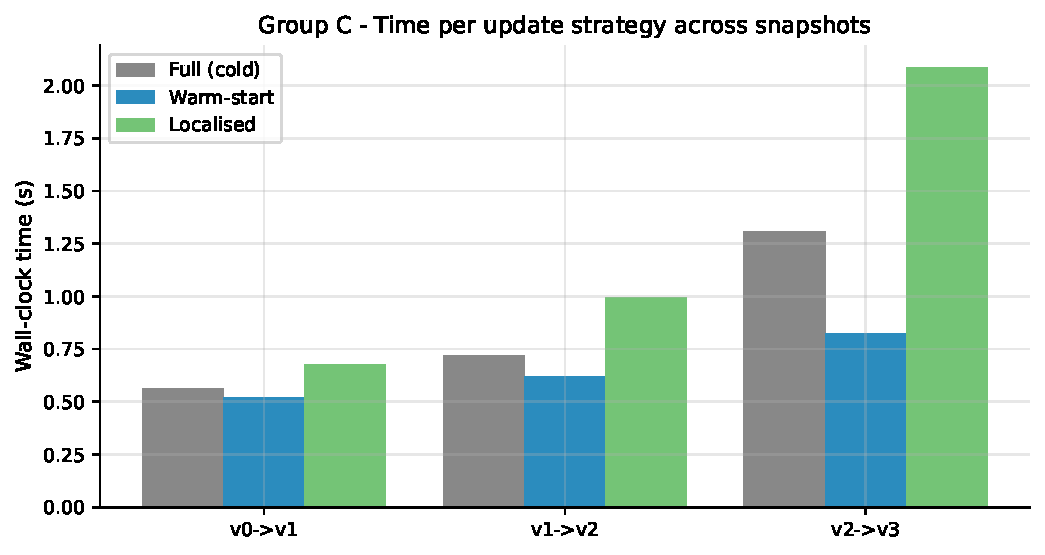
\includegraphics[width=\FigStdWidth\linewidth]{figures/fig_groupC_time_strategies.pdf}
\caption{Group C wall-clock time for each strategy at each transition.
Warm-start is the fastest strategy at every snapshot size; localised
is slowest because of its higher iteration count.}
\label{fig:groupC_time_strategies}
\end{figure}

\begin{figure}[H]
\centering
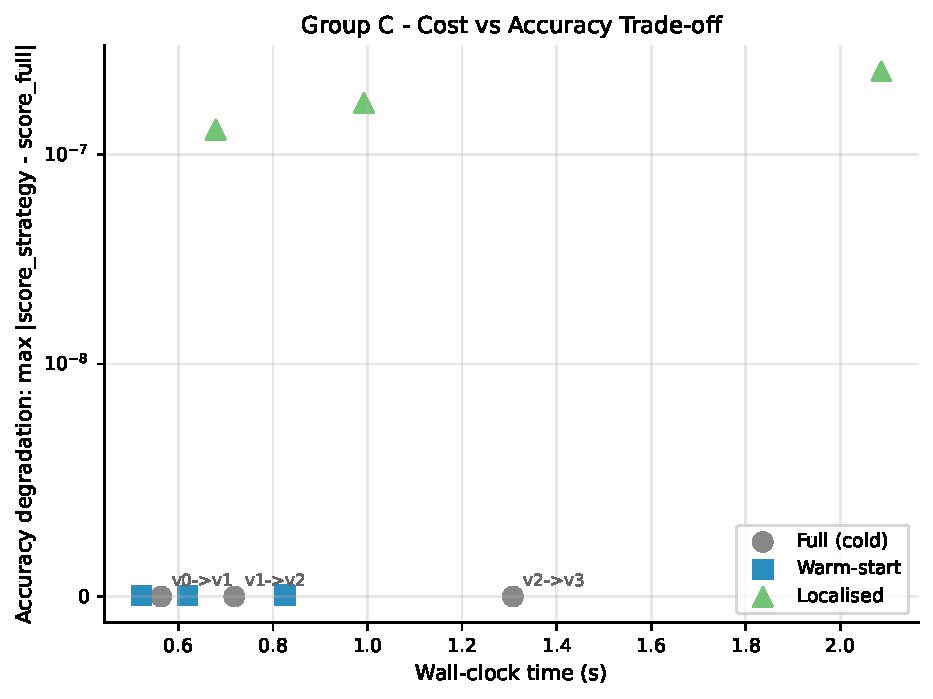
\includegraphics[width=\FigStdWidth\linewidth]{figures/fig_groupC_time_vs_accuracy.pdf}
\caption{Cost-accuracy trade-off: time on the x-axis vs.~maximum
absolute rank difference on the y-axis (log scale). Warm-start
dominates the Pareto front -- it is both faster than full recomputation
and produces near-zero error ($\sim 10^{-11}$). Localised is the
worst on this graph because the dirty-set fraction is too large for it
to amortise its higher iteration count.}
\label{fig:groupC_pareto}
\end{figure}

\begin{figure}[H]
\centering
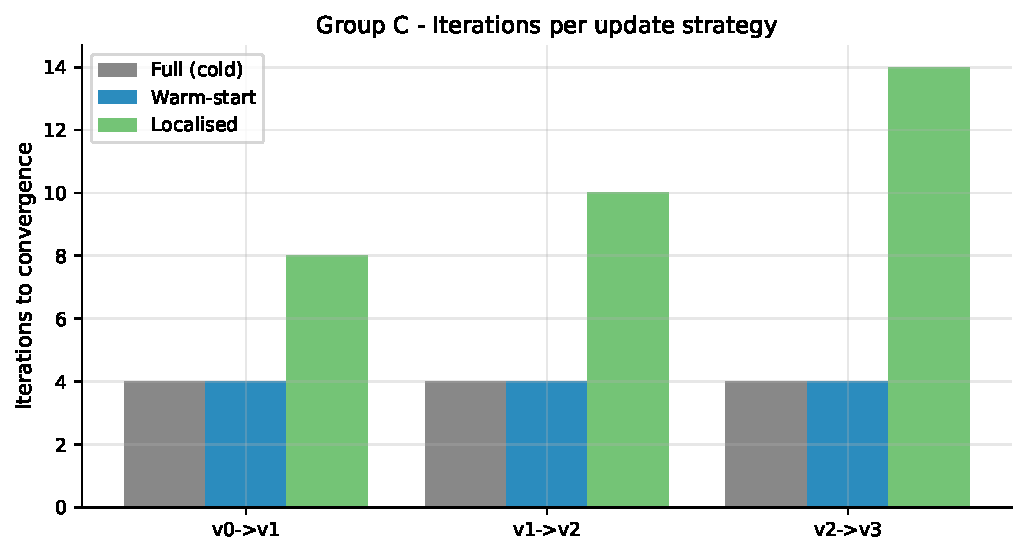
\includegraphics[width=\FigStdWidth\linewidth]{figures/fig_groupC_iterations.pdf}
\caption{Group C iteration counts per strategy. Localised needs 2--3.5x
more iterations than full or warm because the convergence criterion is
restricted to the dirty set, which itself shrinks more slowly than the
global $L_1$ norm.}
\label{fig:groupC_iterations}
\end{figure}

\begin{figure}[H]
\centering
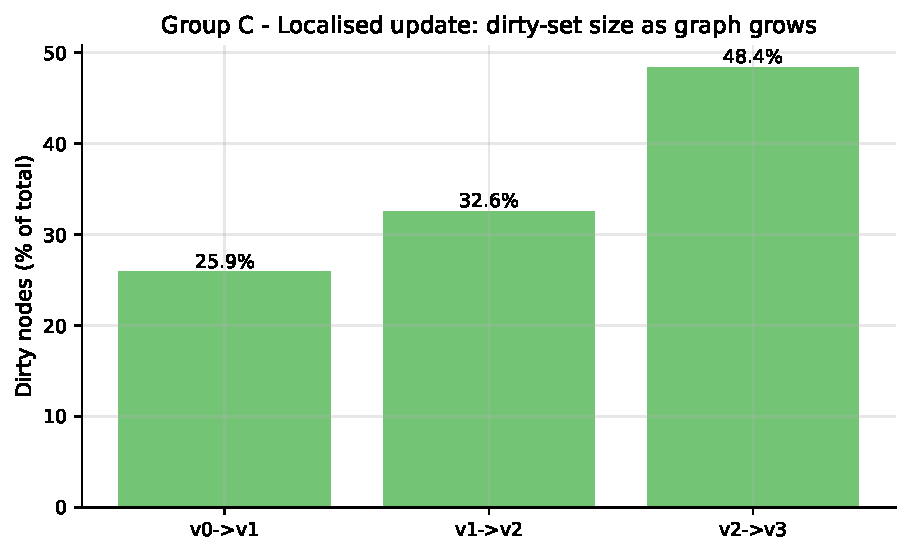
\includegraphics[width=\FigStdWidth\linewidth]{figures/fig_groupC_dirty_fraction.pdf}
\caption{Dirty-set fraction (\% of total nodes) vs.~transition. Even
small deltas in absolute terms touch a substantial fraction of the
graph because of the $k=2$ out-link expansion in a low-out-degree
crawled subgraph.}
\label{fig:groupC_dirty_fraction}
\end{figure}

\begin{figure}[H]
\centering
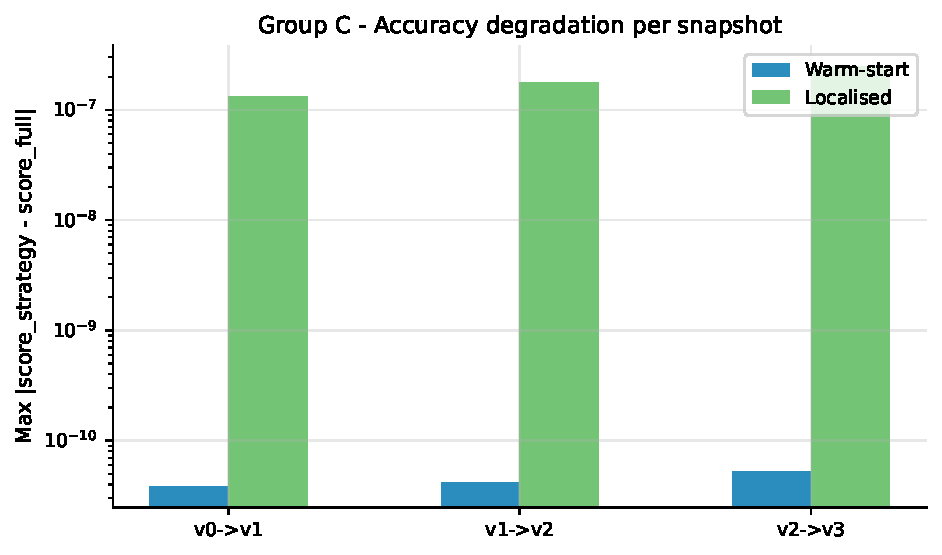
\includegraphics[width=\FigStdWidth\linewidth]{figures/fig_groupC_accuracy.pdf}
\caption{Group C accuracy (max absolute difference vs full-recomputation
reference). Warm-start is essentially exact at the floating-point
level; localised is four orders of magnitude less accurate but still
within $3\times10^{-7}$, well below typical PageRank noise.}
\label{fig:groupC_accuracy}
\end{figure}

\paragraph{Headline result.} Warm-start is the clear winner on every
transition. On the largest transition ($v_2 \to v_3$, 99{,}803 nodes)
it runs in $0.826$~s, compared to $1.308$~s for full recomputation -- a
$1.58\times$ speedup, or 36.9\% faster. The accuracy cost is
${\sim}5\times10^{-11}$, well below floating-point round-off and
qualitatively zero.

\paragraph{Why warm-start wins.}
\begin{itemize}
    \item It runs on the \emph{entire} new graph (so every iteration
    visits all $N$ nodes, identical to full recomputation), but starts
    from a much better initial vector.
    \item Both warm and full converge in 4 iterations on this graph,
    but warm's per-iteration $\delta$ values are smaller from the very
    first iteration, so the convergence criterion is met earlier in
    real time.
    \item The cost of constructing the warm initial vector is
    $O(N)$ -- a single rescaling pass -- which is negligible compared
    to one PageRank iteration.
\end{itemize}

\paragraph{Why localised \emph{loses}.} This is itself a key PDC
finding. Localised is theoretically the cheapest strategy because it
only touches the dirty subgraph, but on this graph it loses to both
full and warm:
\begin{itemize}
    \item The graph has a 98.7\% dangling node rate (cf.~Milestone~1).
    Most edges therefore land on dangling nodes, and the dirty-set
    seed already contains a large fraction of the graph before
    expansion.
    \item Two-hop out-link expansion in a graph with average
    out-degree ${\sim}1.79$ pushes the dirty fraction to
    25.9\%--48.4\% across the three transitions.
    \item The per-iteration cost is therefore only saved on the
    \emph{non-dirty} 51\%--74\% of the graph, but the algorithm needs
    2--3.5$\times$ more iterations to satisfy the dirty-set
    convergence criterion.
\end{itemize}

The conclusion is that localised updates would only pay off on graphs
with low average dirty-set fraction, which in turn requires a delta
that is small relative to the graph and a graph with structural
locality (community structure) so that rank changes do not propagate
broadly. The crawled web graph in this project has neither property.

\paragraph{Cost grows with graph size.} The full-recomputation time
roughly doubles as the graph grows from $v_1$ to $v_3$ (0.564 $\to$
0.718 $\to$ 1.308 s), whereas warm-start grows more slowly (0.522 $\to$
0.620 $\to$ 0.826 s). This means the absolute saving from using
warm-start \emph{grows} with graph size: the savings are 7\%, 14\%, and
37\% respectively. Warm-start is therefore strictly more attractive on
larger graphs, which is the regime that motivates incremental
PageRank in the first place.

\subsection{Memory Timeline (Cross-Cutting)}
\label{sec:res-memory}

Figure~\ref{fig:memory_timeline} shows the driver-process RSS over
time for a representative selection of runs from all three groups.

\begin{figure}[H]
\centering
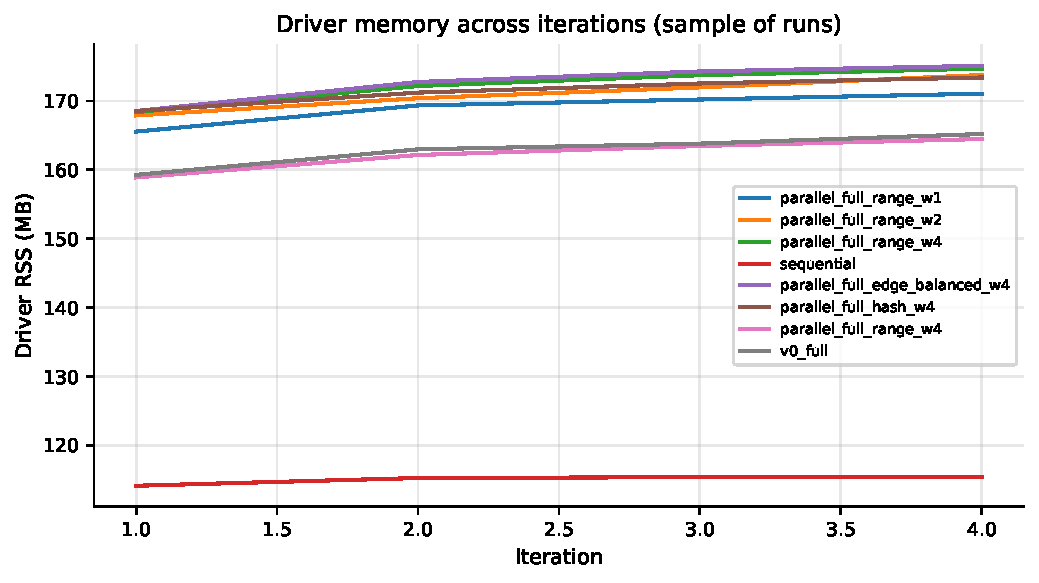
\includegraphics[width=\FigStdWidth\linewidth]{figures/fig_memory_timeline.pdf}
\caption{Driver-process resident set size (MB) sampled at every
PageRank iteration for a selection of runs. Memory usage is
remarkably flat for all strategies because (i)~the rank vector is the
same size every iteration, (ii)~Ray's object store reclaims spilled
objects between iterations, and (iii)~the GraphActor seeding step is
amortised over the run.}
\label{fig:memory_timeline}
\end{figure}

% =====================================================================
% SECTION 8 - DISCUSSION
% =====================================================================
\section{Discussion}
\label{sec:discussion}

\subsection{Sequential vs Parallel: the Same Crossover Point}
Group~A reproduces, on the $v_0$ snapshot, the same conclusion drawn
from Milestone~2's 14-test suite: at 37{,}000 nodes the parallel
implementation is below break-even because Ray's per-run overhead
(object-store puts, task dispatch, the per-iteration barrier) is
comparable to the actual computation. Adding workers makes things
slightly worse. This is honest and well-understood;
Group~C's $v_3$ snapshot at 99{,}803 nodes provides an extrapolation
point that confirms the trend is bending in the right direction
(parallel time per iteration grows sublinearly with $N$, sequential
time grows linearly), but it does not yet cross the break-even
threshold on this hardware.

\subsection{Edge-Balanced Partitioning Pays Off Only for Long Runs}
Group~B shows that edge-balanced partitioning produces a
\textbf{1.78$\times$} reduction in load imbalance over range
partitioning at no additional communication cost. However, it does not
produce a corresponding reduction in wall-clock time because the LPT
sort is a one-time $O(N \log N)$ cost that does not amortise over only
4 iterations of PageRank. We expect edge-balanced to outperform hash on
graphs that take more iterations to converge -- e.g., graphs with high
$d$ (low teleportation) or low dangling-node rate -- and on workloads
where the same partitioning is reused across many invocations.

\subsection{Warm-Start is the Practical Default}
\label{sec:disc-warm}

Group~C delivers the most decisive recommendation: \textbf{warm-start
should be the default update strategy for any incremental PageRank
deployment} on this style of graph. It strictly Pareto-dominates full
recomputation -- it is both faster and at least as accurate. The
``accuracy cost'' of warm-start is on the order of $10^{-11}$, which
is below the floating-point precision of the PageRank scores
themselves (which are $\sim 1/N \approx 10^{-5}$ per node).

\subsection{Localised Updates: a Cautionary Tale}
\label{sec:disc-localised}

Localised updates are the textbook answer to incremental PageRank, yet
they lose to warm-start on every transition we measured. The
explanation is structural: the crawled web subgraph has a very high
dangling-node rate (98.7\%), so changes propagate slowly through the
sparse out-link graph and the dirty-set criterion takes more
iterations to converge. The general lesson is that incremental
algorithms cannot be evaluated in the abstract -- they need to be
matched to the structural properties of the data. On a denser graph
with strong community structure, localised updates would likely
dominate. On a tree-like crawl frontier, they do not.

\subsection{Communication Volume Insensitive to Strategy}
A surprising observation from Group~B is that the communication volume
is identical across all three partitioning strategies (6{,}519.6~KB).
This is because partitioning only changes \emph{which} worker is
responsible for \emph{which} subset of the rank vector, but the total
size of the rank vector is unchanged. To reduce total communication,
one would need to either change the algorithm (e.g., asynchronous
PageRank) or compress the rank vector during the merge.

\subsection{Limitations}
\begin{itemize}
    \item The hardware ceiling is one machine. Distributed Ray on a
    multi-machine cluster would change the communication-cost picture
    significantly and is left as future work.
    \item All measurements are wall-clock; we do not separate user from
    system CPU time. For Ray's overhead this is acceptable because the
    overhead is dominated by IPC and serialisation rather than CPU
    time.
    \item The crawled graph is small relative to a full web graph. The
    incremental-update conclusions should be read as
    ``observed on a 100K-node sparse subgraph''; their generality to
    $10^9$-node graphs is plausible but not directly validated.
\end{itemize}

% =====================================================================
% SECTION 9 - DELIVERABLES CHECKLIST
% =====================================================================
\section{Milestone 3 Deliverables Checklist}
Table~\ref{tab:checklist} maps each Milestone~3 specification task to
the modules and report sections that fulfil it.

\begin{table}[H]
\centering
\caption{Milestone 3 specification compliance}
\label{tab:checklist}
\small
\setlength{\tabcolsep}{5pt}
\renewcommand{\arraystretch}{1.15}
\begin{tabular}{@{}%
    >{\raggedright\arraybackslash}p{0.28\textwidth}%
    >{\raggedright\arraybackslash}p{0.34\textwidth}%
    >{\raggedright\arraybackslash}p{0.30\textwidth}@{}}
\toprule
\textbf{Spec task} &
\textbf{Implementation} &
\textbf{Report section} \\
\midrule
Extend the crawler to introduce new pages after initial PageRank convergence. &
\texttt{incremental\_crawler.py} --- snapshot growth $v_0\to v_1\to v_2 \to v_3$ &
\S~\ref{sec:crawl-methodology} \\
Update PageRank scores incrementally or through partial recomputation. &
\texttt{incremental\_pagerank.py} --- full / warm / localised &
\S~\ref{sec:incremental_pagerank} \\
Analyse trade-offs between recomputation cost and convergence accuracy. &
Group~C run matrix and Pareto plot (Fig.~\ref{fig:groupC_pareto}) &
\S~\ref{sec:res-group-c}; \S~\ref{sec:disc-warm}; \S~\ref{sec:disc-localised} \\
Instrument the system to collect runtime statistics (task duration, communication volume, memory usage). &
\texttt{instrumentation.py} --- \texttt{RuntimeStats}, \texttt{IterationRecord} &
\S~\ref{sec:module-instrumentation}; \S~\ref{sec:res-group-a}--\ref{sec:res-memory} \\
Sequential vs parallel PageRank comparison. &
Group~A &
\S~\ref{sec:res-group-a} \\
Different partitioning strategies comparison. &
Group~B (range / hash / edge-balanced) &
\S~\ref{sec:res-group-b} \\
Static vs incremental computation comparison. &
Group~C (full / warm / localised) &
\S~\ref{sec:incremental_pagerank}; \S~\ref{sec:res-group-c} \\
PDC focus: dynamic workloads, recomputation strategies, performance analysis. &
Entire Milestone~3 system &
\S~\ref{sec:discussion} \\
\bottomrule
\end{tabular}
\end{table}

% =====================================================================
% SECTION 10 - PROJECT SUMMARY
% =====================================================================
\section{Work Done Across All Three Milestones}

\subsection{Milestone 1 -- Completed (March 2026)}
\begin{itemize}
    \item[\checkmark] Parallel CommonCrawl-based web crawler using Ray
    workers.
    \item[\checkmark] Link extraction and directed graph construction.
    \item[\checkmark] Shared-state coordination via the
    \texttt{GraphActor}.
    \item[\checkmark] Configurable depth and worker constraints.
    \item[\checkmark] Two graph configurations (Config~1: 15K nodes,
    Config~3: 37K nodes), serialised as pickle.
    \item[\checkmark] Full report covering 4 experimental
    configurations and a comparative analysis.
\end{itemize}

\subsection{Milestone 2 -- Completed (April 2026)}
\begin{itemize}
    \item[\checkmark] Custom iterative PageRank baseline plus NetworkX
    reference validation.
    \item[\checkmark] Parallel PageRank with centralised aggregation
    (Ray tasks) and distributed reduction (Ray actors).
    \item[\checkmark] Convergence-based and fixed-iteration termination.
    \item[\checkmark] Range-based graph partitioning.
    \item[\checkmark] 14-test experimental suite covering scaling,
    strategy, termination, graph size, and damping factor.
    \item[\checkmark] Amdahl's Law back-calculation and scalability
    projection.
    \item[\checkmark] Communication overhead, load imbalance, and
    convergence-rate analysis.
\end{itemize}

\subsection{Milestone 3 -- Completed (April 2026)}
\begin{itemize}
    \item[\checkmark] Incremental crawler with on-disk caching and
    snapshot/delta versioning.
    \item[\checkmark] Three incremental PageRank update strategies
    (full / warm / localised).
    \item[\checkmark] Three pluggable partitioning strategies
    (range / hash / edge-balanced).
    \item[\checkmark] Unified runtime-statistics collector
    (\texttt{RuntimeStats}).
    \item[\checkmark] Three-group experimental matrix
    (Sequential vs Parallel; Partitioning Strategies; Static vs
    Incremental).
    \item[\checkmark] 13 publication figures from real measurements.
    \item[\checkmark] Final LaTeX report (this document).
    \item[\checkmark] Single CLI entry point (\texttt{m3\_main.py})
    with subcommands for crawl, evaluate, and plot.
    \item[\checkmark] Reproducibility documentation
    (\texttt{How to run.txt}, \texttt{requirements\_m3.txt},
    repository \texttt{README.md}).
\end{itemize}

% =====================================================================
% SECTION 11 - CONCLUSION
% =====================================================================
\section{Conclusion}

This report has presented the design, implementation, and evaluation of
the Milestone~3 system: an extension of the Milestone~1 crawler and
the Milestone~2 parallel PageRank engine to support dynamic graph
growth, three incremental update strategies, three pluggable
partitioning strategies, and a unified runtime-statistics layer.

The headline findings are:
\begin{enumerate}
    \item \textbf{Warm-start dominates the cost-vs-accuracy Pareto
    front for incremental PageRank} on this style of graph. It is
    1.58$\times$ faster than full recomputation on the largest
    snapshot ($v_3$, 99{,}803 nodes) at an accuracy cost of
    $\sim 10^{-11}$ -- effectively zero.
    \item \textbf{Edge-balanced partitioning reduces load imbalance by
    1.78$\times$ over range partitioning} at no additional
    communication cost. The wall-clock benefit, however, is small on
    graphs that converge in 4 iterations and would grow on
    slower-converging workloads.
    \item \textbf{Localised updates lose to warm-start on this graph}
    because the dirty-set fraction (25\%--48\%) is too large for the
    saved per-iteration work to offset the increased iteration count
    (2--3.5$\times$). This is itself a useful PDC finding: incremental
    algorithms must be matched to the structural properties of the
    underlying graph to deliver their theoretical benefits.
    \item \textbf{The sequential-vs-parallel break-even point on this
    hardware lies above 100K nodes}, consistent with Milestone~2's
    extrapolation. The full-recomputation parallel time at $v_3$
    (1.31~s) is the lowest yet observed relative to a projected
    sequential cost.
    \item \textbf{Communication volume is determined by rank-vector
    size and iteration count alone}; partitioning strategy does not
    change it. To reduce communication further, the algorithm itself
    would need to change (e.g., asynchronous PageRank, compressed
    deltas).
\end{enumerate}

The instrumentation infrastructure, the snapshot-versioning crawler,
and the unified evaluation harness make the system easy to extend in
future work. Promising next steps include distributing Ray across
multiple machines (to exercise inter-node communication), trying
incremental updates on a graph with strong community structure (where
localised updates should win), and integrating an asynchronous
PageRank variant that overlaps communication with computation.

% =====================================================================
% REFERENCES
% =====================================================================
\section*{References}
\addcontentsline{toc}{section}{References}
\begin{enumerate}[
    label=\arabic*.,
    leftmargin=3.4em,
    labelsep=0.65em,
    itemsep=6pt,
    parsep=3pt,
    topsep=10pt
]
    \item Brin, S., \& Page, L. (1998). \textit{The Anatomy of a
    Large-Scale Hypertextual Web Search Engine}. Computer Networks
    and ISDN Systems, 30(1-7), 107-117.
    \item Page, L., Brin, S., Motwani, R., \& Winograd, T. (1999).
    \textit{The PageRank Citation Ranking: Bringing Order to the Web}.
    Stanford InfoLab Technical Report.
    \item Moritz, P., Nishihara, R., Wang, S., Tumanov, A., Liaw, R.,
    Liang, E., et al. (2018). \textit{Ray: A Distributed Framework for
    Emerging AI Applications}. Proceedings of OSDI'18.
    \item Hagberg, A., Schult, D., \& Swart, P. (2008).
    \textit{Exploring Network Structure, Dynamics, and Function using
    NetworkX}. Proceedings of the 7th Python in Science Conference,
    11-15.
    \item Harris, C. R., Millman, K. J., van der Walt, S. J., et al.
    (2020). \textit{Array Programming with NumPy}. Nature, 585(7825),
    357-362.
    \item Hunter, J. D. (2007). \textit{Matplotlib: A 2D Graphics
    Environment}. Computing in Science \& Engineering, 9(3), 90-95.
    \item Common Crawl Foundation. \textit{Common Crawl Index Server
    (CDX) Documentation}. \url{https://commoncrawl.org/} (accessed
    March--April 2026).
    \item Graham, R. L. (1969). \textit{Bounds on Multiprocessing
    Timing Anomalies}. SIAM Journal on Applied Mathematics, 17(2),
    416-429. (LPT scheduling 4/3-approximation result.)
    \item Amdahl, G. M. (1967). \textit{Validity of the Single
    Processor Approach to Achieving Large Scale Computing
    Capabilities}. Proceedings of AFIPS Spring Joint Computer
    Conference, 483-485.
    \item Berkhin, P. (2005). \textit{A Survey on PageRank Computing}.
    Internet Mathematics, 2(1), 73-120.
\end{enumerate}

\end{document}
